% Study 2. Numbers come from results/study2/study2_results.txt,
% results/study2/trajectory/study2_trajectory_results.txt and
% results/study2/preference/study2_preference_results.txt.

\section{Study 2}
\label{sec:study2}

Study~1 showed that both trajectory visualizations reduced VIMS relative to
unmodified 360$^\circ$ video while costing less Presence than Dynamic FOV.
However, Study~1 compared them with only one other mitigation technique and
measured sickness only after each trial. Study~2 therefore compared our
\textit{Minimap} and \textit{Overlay Path} interfaces with \textit{Reverse
Optical Flow} (ROF), a counter-optical-flow visualization. We treated Minimap
and Overlay Path as the \emph{trajectory-based} interfaces and ROF as the
\emph{non-trajectory} comparison, and asked: \textbf{are trajectory-based
interfaces as effective as ROF at reducing VIMS, while being less intrusive?}
Study~2 also measured sickness both before and after every trial, and
collected a complete preference ranking and interview from every participant.

\subsection{Participants}

We recruited 36 participants. % TODO: age range, gender, and whether any also took part in Study 1.
Nineteen had used a VR headset before and 17 had not. All participants
completed all nine experimental conditions (three methods $\times$ three
videos), yielding 324 trials and 648 SSQ administrations with no missing data.

\subsection{Study Design and Procedure}

Study~2 followed a 3 (\textit{Method}: ROF, Minimap, Overlay Path) $\times$ 3
(\textit{Video}: Walking, Cycling, Driving) within-subjects design. Unlike
Study~1, it had \textbf{no Baseline condition}, so all comparisons are between
mitigation techniques. Each participant experienced the three methods in
separate blocks, and each block contained all three videos. Method order was
fully counterbalanced: each of the six possible orders was assigned to six
participants. Video order within blocks was counterbalanced so that each video
appeared equally often in each position. Participants completed the SSQ
immediately before each video, and the SSQ and the Presence questionnaire
immediately after it. The median interval between finishing one trial and
starting the next was 6.3 minutes (IQR 5.1--7.3). After all nine trials,
participants ranked the three methods and took part in a short interview.

\subsection{Measures}

\paragraph{Simulator sickness.}
We used the same Vietnamese version of the 16-item SSQ and the same Kennedy
weighted scores (TSC, N, O, D) as in Study~1, but administered the
questionnaire both before and after every trial. Our main outcome was the
change score $\Delta = \text{post} - \text{pre}$, where positive values mean
that symptoms increased during viewing. The pre-trial scores also let us check
that participants started each condition at a similar level of sickness.

\paragraph{Immersion.}
Participants completed the same five-item, 7-point presence questionnaire as in
Study~1 after every trial (Cronbach's $\alpha = .78$).

\paragraph{Preference ranking and post-study interviews.}
After all nine trials, every participant ranked the three methods from 1 (best)
to 3 by how well each balanced immersion and VIMS mitigation, and explained the
ranking in a semi-structured interview. Later participants were also asked
which method best reduced their sickness (21 named one method) and which felt
most realistic (26 named one method). We coded the interview notes with a
codebook of eleven codes in three families: \emph{perceived sickness},
\emph{perceived realism}, and \emph{interface experience} (occlusion,
distraction, glance cost, route anticipation, timing, visual noise, visibility,
familiarity, and agency). Each code was counted at most once per participant
and method, so all counts below are numbers of participants.

To address intrusiveness, we counted a \emph{recorded intrusiveness-related
complaint} when a participant criticized a method for blocking the scene
(occlusion), drawing attention away from it (distraction), requiring gaze
shifts (glance cost), or producing flicker or visual clutter (visual noise).
Participants were not asked directly whether a method was intrusive, so this
measure counts unprompted complaints; a method without complaints is not
thereby shown to be unobtrusive.

\subsection{Analysis}

For the SSQ, we conducted 2 (\textit{Time}: pre, post) $\times$ 3
(\textit{Method}) $\times$ 3 (\textit{Video}) repeated-measures ANOVAs.
The \textit{Time} $\times$ \textit{Method} interaction is the effect of
interest, because it tests whether the methods differed in how much sickness
increased during viewing. As in Study~1, we applied Greenhouse--Geisser
corrections, Holm corrections across the four SSQ outcomes, and report
$\eta^2_G$. Presence was analyzed with a 3 $\times$ 3 repeated-measures ANOVA.

To compare the trajectory-based interfaces with ROF, we computed for each
participant the difference between their mean $\Delta$TSC under Minimap and
Overlay Path and their $\Delta$TSC under ROF (contrast weights
$-1, \frac{1}{2}, \frac{1}{2}$). Because the question is whether the
trajectory-based interfaces are \emph{as effective as} ROF, we used a
\textbf{non-inferiority test} (one-sided $\alpha = .05$) with a margin of
$+5$ TSC points: the trajectory-based interfaces are non-inferior if the upper
limit of the 90\% confidence interval of the difference lies below $+5$. The
margin is one third of the smallest reduction relative to Baseline in Study~1
(14.9 TSC points, Overlay Path), so a non-inferior method keeps at least
two-thirds of that benefit. We checked the result with a mixed-effects model on
all 324 trials, a participant bootstrap, and separate tests for each
trajectory-based interface.

For intrusiveness, we computed for each participant the difference between
whether they complained about ROF (0 or 1) and the mean of the same indicator
for Minimap and Overlay Path. We tested whether this difference was positive
with an exact permutation test that enumerates every assignment of the three
method labels within each participant. Answering the research question in the
affirmative required both the non-inferiority test and the intrusiveness test
to be significant; because both must succeed, no further $\alpha$ adjustment is
needed.

For the ranking, we used a Friedman test with Kendall's $W$, and a
Plackett--Luce model in which Minimap and Overlay Path share one preference
parameter.

The SSQ change scores were zero-inflated and heavy-tailed. Rank-transformed
ANOVAs, Friedman tests, bootstrap confidence intervals, and a mixed model
excluding extreme values all led to the same conclusions, so we report the
parametric results below.

\subsection{Results}

\subsubsection{VIMS and SSQ}

Table~\ref{tab:s2-anova} summarizes the ANOVA results and
Table~\ref{tab:s2-means} the scores for each method. \textbf{Viewing increased
sickness under every method}: \textit{Time} was significant for all four SSQ
outcomes, and TSC rose from 9.55 before to 17.98 after viewing (+8.44, 95\% CI
[5.27, 11.61], $d_z = 0.90$). \textbf{The method did not affect how much
sickness increased}: the \textit{Time} $\times$ \textit{Method} interaction was
not significant for any SSQ outcome (all $F \le 0.78$, uncorrected
$p \ge .44$, $\eta^2_G \le .001$). As Figure~\ref{fig:s2-prepost} shows, TSC
increased by 9.00 points with ROF, 9.07 with Minimap, and 7.24 with Overlay
Path. Participants started each method at a similar level (pre-trial TSC 9.90,
9.38, and 9.35; all $p \ge .77$), so these differences reflect what happened
during viewing.

The \textbf{video type} mattered more than the method. The \textit{Time}
$\times$ \textit{Video} interaction was significant for TSC, Oculomotor
discomfort, and Disorientation: the Walking video increased TSC by 13.09
points, roughly 2.4 times the increase for Driving (5.44) and nearly twice that
for Cycling (6.79). Walking differed from both other videos (Bonferroni
$p \le .003$), whereas Cycling and Driving did not differ. The three-way
interaction was not significant, so no method was better suited to a
particular video.

Symptoms partly carried over between trials: the post-trial TSC of one trial
predicted the pre-trial TSC of the next ($b = 0.39$, $p < .001$). Because
method order was fully counterbalanced, this carryover adds noise but does not
favor any method.

\begin{table*}[t]
  \caption{Repeated-measures ANOVA results for Study~2. SSQ outcomes were
  analyzed with a 2 (Time) $\times$ 3 (Method) $\times$ 3 (Video) ANOVA;
  Presence, measured after viewing only, with a 3 (Method) $\times$ 3 (Video)
  ANOVA. $F$ values are reported for significant effects;
  Greenhouse--Geisser corrections were applied, and $p$ values for the SSQ
  outcomes are Holm-corrected across the four outcomes. Time: $df = 1, 35$.}
  \label{tab:s2-anova}
  \centering
  \footnotesize
  \begin{tabular}{lccccc}
    \toprule
    \textbf{Effect} & \textbf{TSC} & \textbf{Nausea} & \textbf{Oculomotor} & \textbf{Disorientation} & \textbf{Presence} \\
    \midrule
    Time                          & $F = 29.15$, $p < .001$ & $F = 11.08$, $p = .002$ & $F = 23.97$, $p < .001$ & $F = 28.64$, $p < .001$ & -- \\
    Method                        & $p = 1.000$ & $p = 1.000$ & $p = 1.000$ & $p = 1.000$ & $p = .758$ \\
    Video                         & $p = .101$ & $p = .253$ & $F = 5.72$, $p = .021$ & $p = .192$ & $p = .311$ \\
    \textbf{Time $\times$ Method} & $p = 1.000$ & $p = 1.000$ & $p = 1.000$ & $p = 1.000$ & -- \\
    Time $\times$ Video           & $F = 7.73$, $p = .004$ & $p = .060$ & $F = 9.61$, $p = .001$ & $F = 6.91$, $p = .008$ & -- \\
    Method $\times$ Video         & $p = 1.000$ & $p = 1.000$ & $p = 1.000$ & $p = 1.000$ & $p = .568$ \\
    Time $\times$ Method $\times$ Video & $p = 1.000$ & $p = 1.000$ & $p = 1.000$ & $p = 1.000$ & -- \\
    \bottomrule
  \end{tabular}
\end{table*}

\begin{table*}[t]
  \caption{Main quantitative results of Study~2 by method, collapsed across
  video type (participant means $\pm$ SD, $n = 36$). $\Delta$ is the
  post-minus-pre change; positive values mean symptoms increased during
  viewing.}
  \label{tab:s2-means}
  \centering
  \footnotesize
  \begin{tabular}{lccccccc}
    \toprule
    \textbf{Method} & \textbf{Pre TSC} & \textbf{Post TSC} & \textbf{$\Delta$TSC} & \textbf{$\Delta$Nausea} & \textbf{$\Delta$Oculomotor} & \textbf{$\Delta$Disorientation} & \textbf{Presence} \\
    \midrule
    ROF          & $9.90 \pm 18.65$ & $18.91 \pm 21.18$ & $9.00 \pm 9.56$  & $3.97 \pm 6.24$ & $7.65 \pm 9.86$  & $13.66 \pm 15.45$ & $5.10 \pm 1.04$ \\
    Minimap      & $9.38 \pm 15.02$ & $18.46 \pm 20.51$ & $9.07 \pm 11.39$ & $3.27 \pm 9.33$ & $8.91 \pm 11.83$ & $12.63 \pm 16.32$ & $5.12 \pm 1.05$ \\
    Overlay Path & $9.35 \pm 19.45$ & $16.59 \pm 21.59$ & $7.24 \pm 12.60$ & $2.56 \pm 7.93$ & $6.67 \pm 12.28$ & $10.96 \pm 17.22$ & $5.04 \pm 1.06$ \\
    \bottomrule
  \end{tabular}
\end{table*}

\begin{figure*}[t]
  \centering
  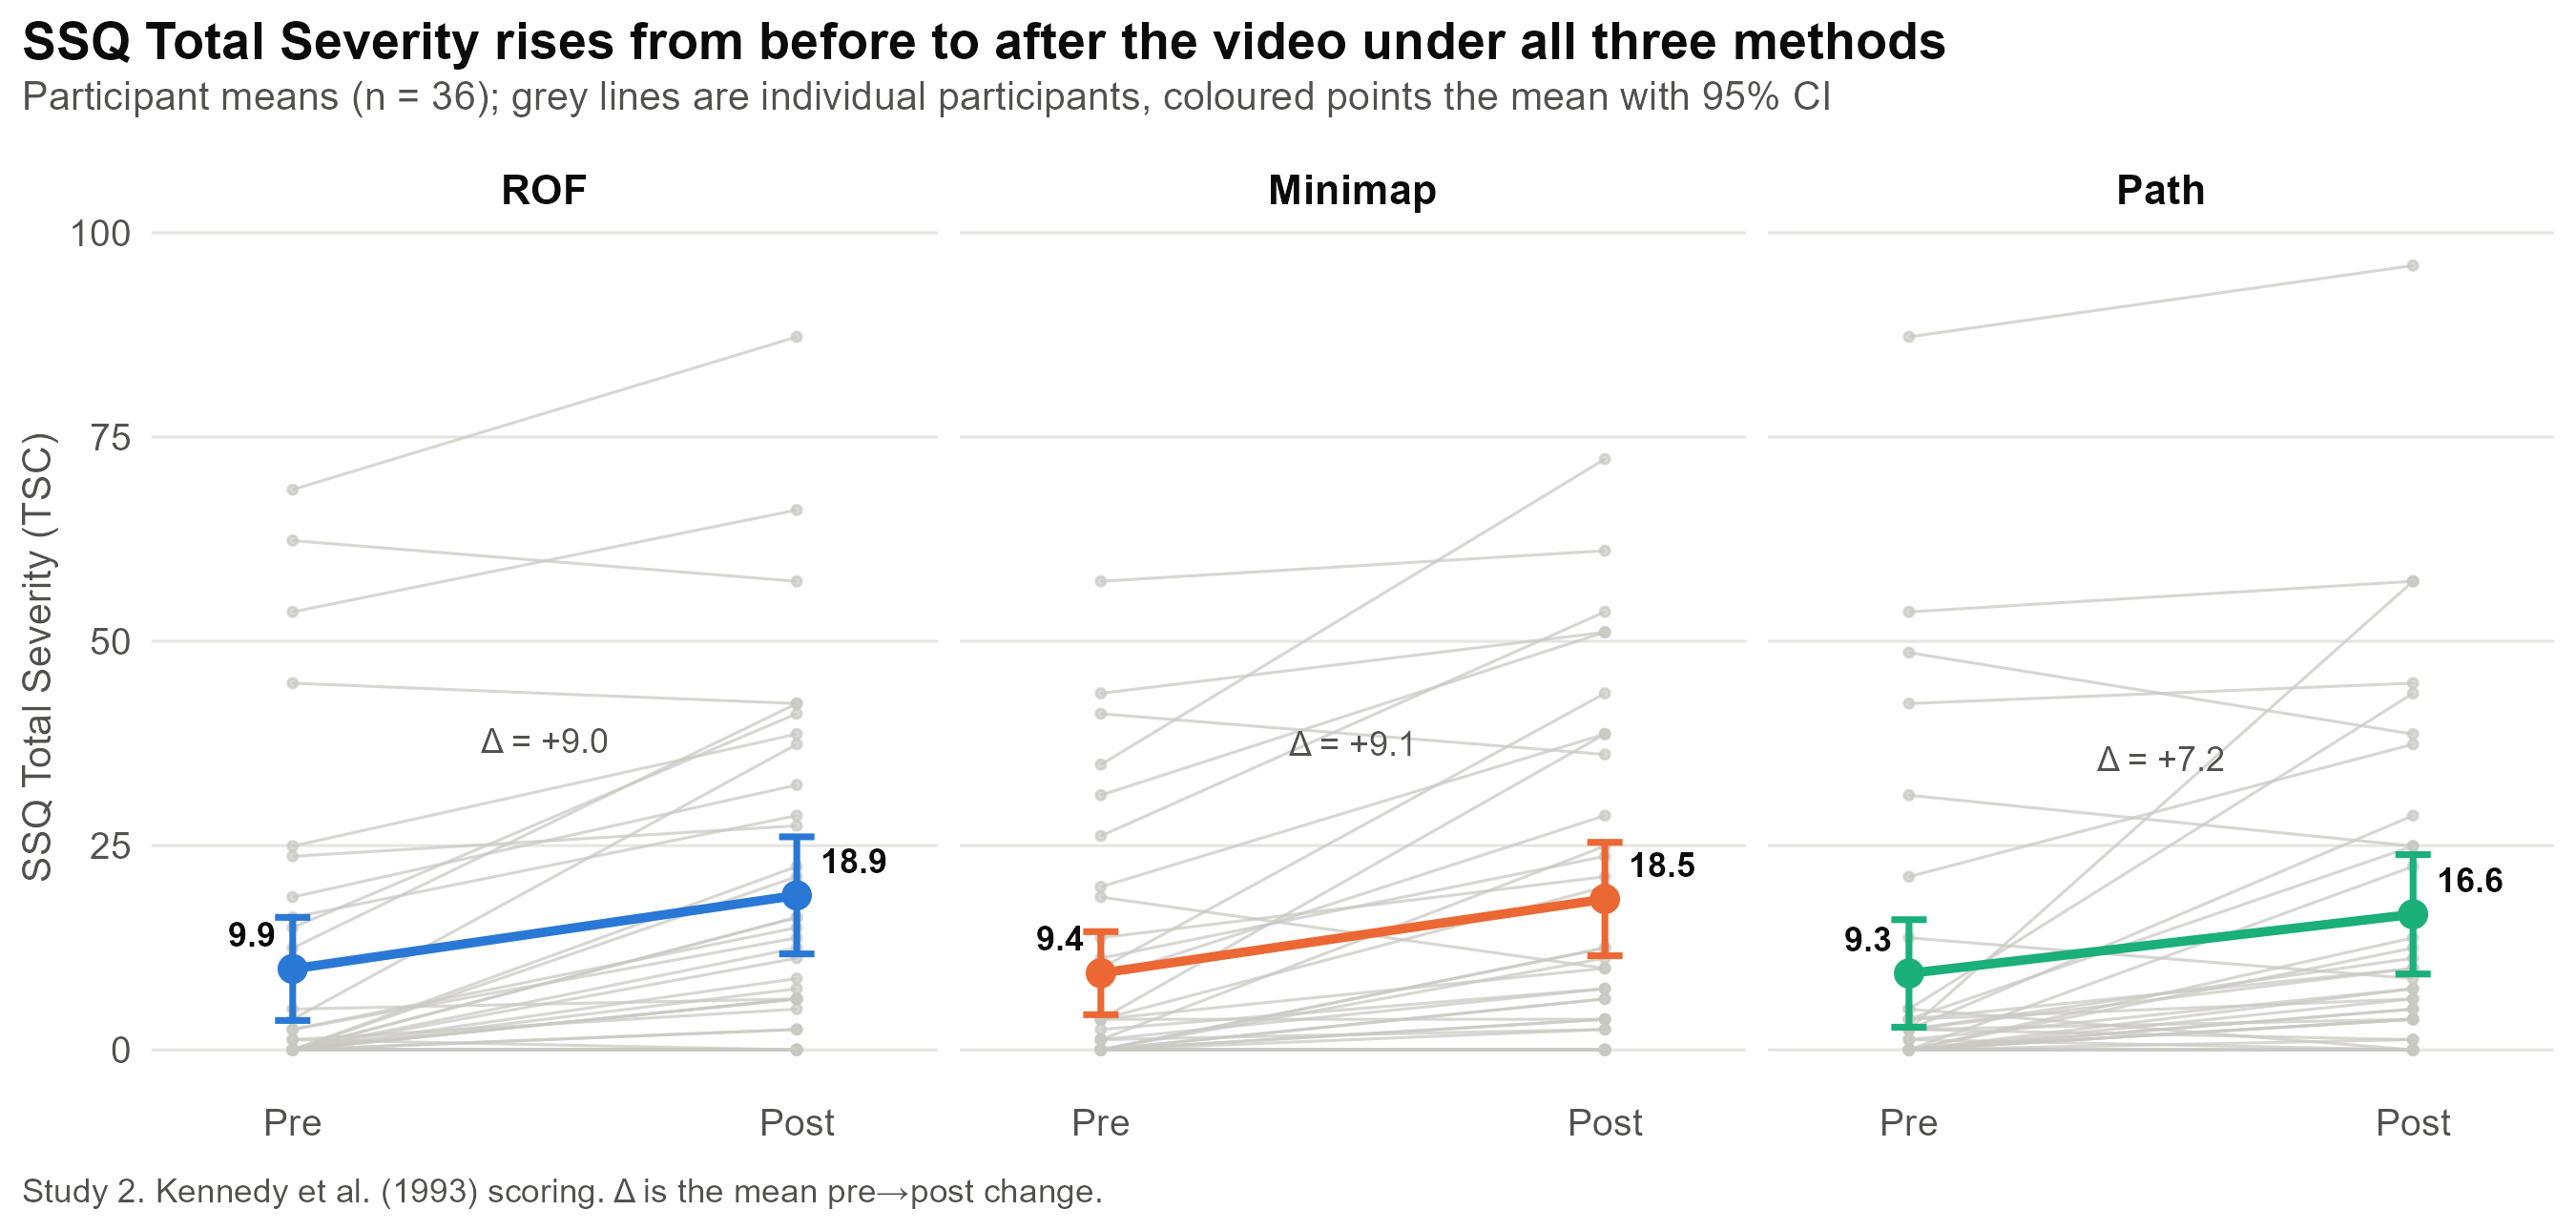
\includegraphics[width=\textwidth]{figures/study2_pre_post_tsc.png}
  \caption{SSQ Total Severity before and after each video in Study~2. Grey
  lines are individual participants (means over the three videos); colored
  points show the mean with 95\% CI. Sickness rose by a similar amount under
  all three methods.}
  \label{fig:s2-prepost}
\end{figure*}

\subsubsection{Are Trajectory-Based Interfaces as Effective as ROF?}

Table~\ref{tab:s2-ni} and Figure~\ref{fig:s2-ni} show the non-inferiority
results. \textbf{The trajectory-based interfaces were non-inferior to ROF in
measured VIMS.} On average, TSC increased 0.85 points \emph{less} with the
trajectory-based interfaces than with ROF (90\% CI [$-2.54$, 0.84]). The upper
limit was well below the $+5$ margin ($p < .001$), and the result held in the
mixed-effects model (upper limit 2.41) and the bootstrap (0.76).
\textbf{Both interfaces were individually non-inferior}: the upper limit was
2.71 for Minimap and 0.69 for Overlay Path (Holm-corrected $p \le .002$). The
difference also lay within $\pm 5$ points in a two-sided equivalence test, so
the trajectory-based interfaces were not meaningfully \emph{better} than ROF
either. No SSQ subscale differed between the groups (all Holm-corrected
$p \ge .83$), and the contrast did not vary by video
($F(1.73, 60.71) = 0.82$, $p = .43$).

Because Study~2 has no Baseline, this result shows that the trajectory-based
interfaces were about as effective as ROF; it does not show that any of the
three methods reduced VIMS relative to unmodified 360$^\circ$ video.

\paragraph{Comparison with Study 1.}
Applying the same contrast to Study~1, with Dynamic FOV as the non-trajectory
comparison, did not establish non-inferiority: post-trial TSC was 7.8 points
higher with the trajectory-based interfaces than with Dynamic FOV (95\% CI
[$-0.9$, 16.5]). This interval includes both zero and the margin, so the
comparison is inconclusive. In Study~1, the trajectory-based interfaces still
reduced TSC by 15.5 points relative to Baseline (95\% CI [6.5, 24.4]) and
produced higher Presence than Dynamic FOV ($+0.55$, 95\% CI [0.26, 0.84]).

\begin{table}[t]
  \caption{Non-inferiority of the trajectory-based interfaces. Difference in
  TSC points (trajectory minus comparison; positive = more sickness).
  Non-inferior when the upper limit of the 90\% CI is below the $+5$ margin.
  Study~2 uses the pre-to-post change; Study~1 uses post-trial TSC.}
  \label{tab:s2-ni}
  \centering
  \footnotesize
  \begin{tabular}{lccc}
    \toprule
    \textbf{Comparison} & \textbf{Difference} & \textbf{90\% CI} & \textbf{Non-inferior} \\
    \midrule
    \multicolumn{4}{l}{\textit{Study 2 (vs ROF)}} \\
    Trajectory (pooled) & $-0.85$ & [$-2.54$, 0.84] & \textbf{yes} \\
    Minimap             & $+0.07$ & [$-2.57$, 2.71] & \textbf{yes} \\
    Overlay Path        & $-1.77$ & [$-4.22$, 0.69] & \textbf{yes} \\
    \midrule
    \multicolumn{4}{l}{\textit{Study 1 (vs Dynamic FOV)}} \\
    Trajectory (pooled) & $+7.81$ & [0.54, 15.08]   & no \\
    Minimap             & $+7.20$ & [0.16, 14.25]   & no \\
    Overlay Path        & $+8.42$ & [$-0.08$, 16.91] & no \\
    \bottomrule
  \end{tabular}
\end{table}

\begin{figure*}[t]
  \centering
  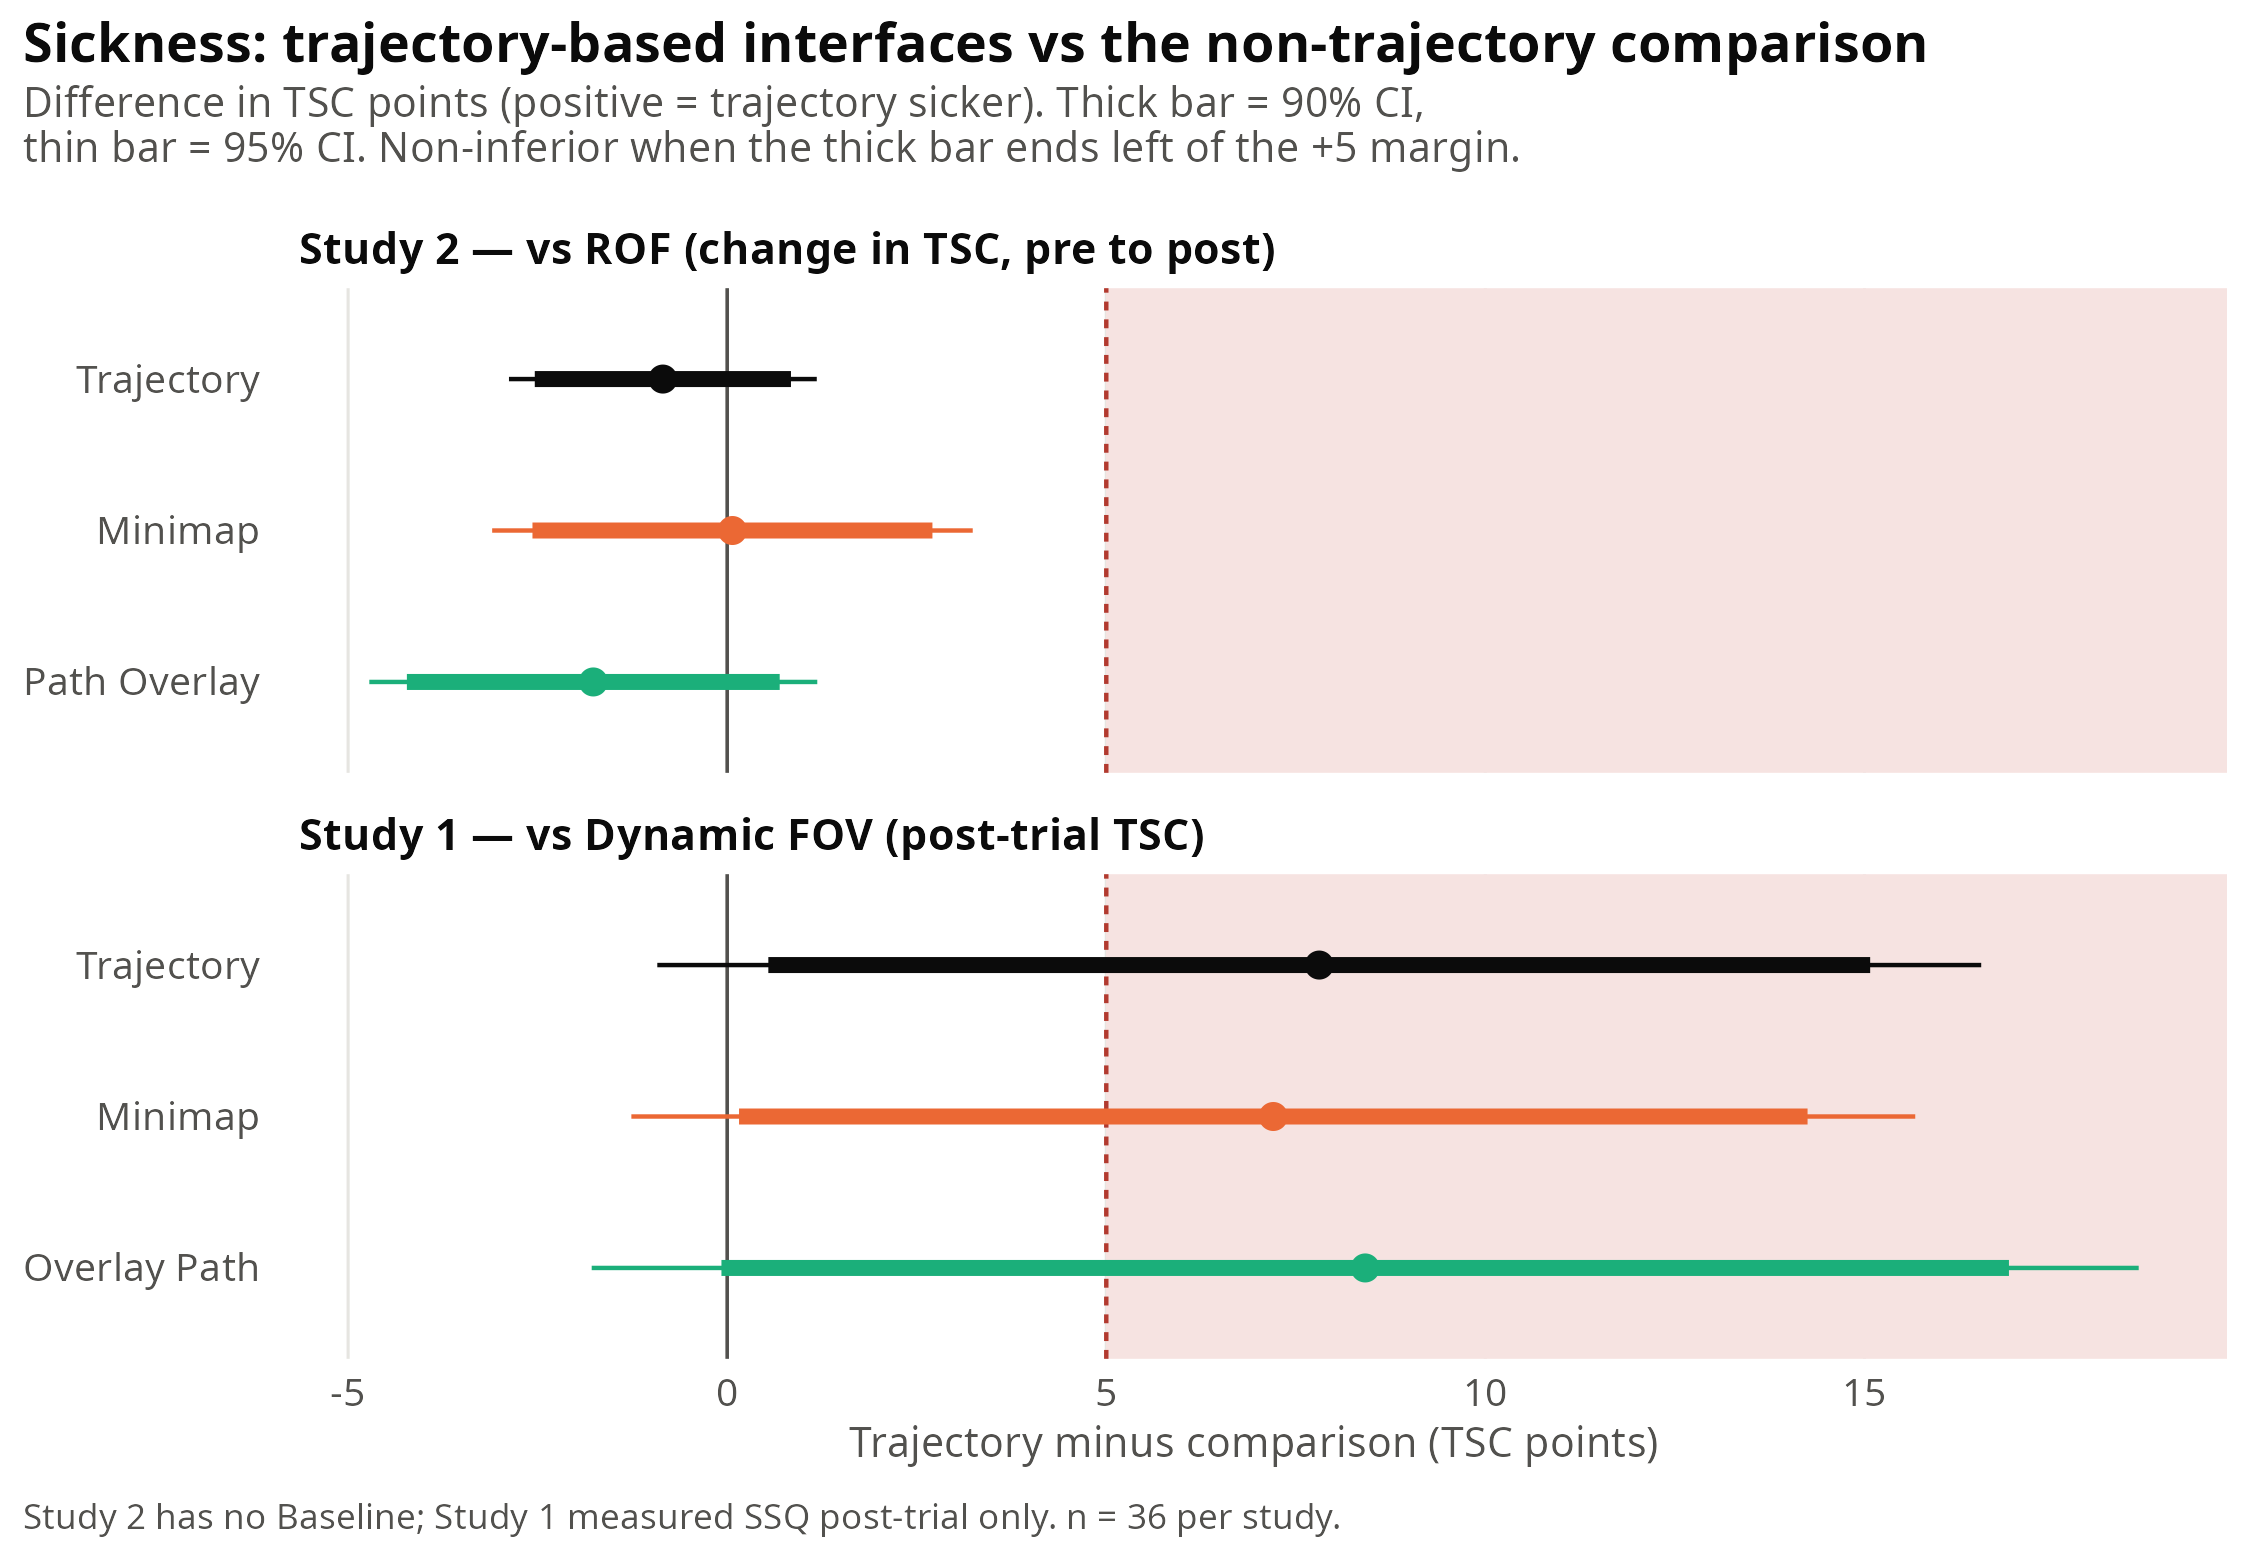
\includegraphics[width=0.8\textwidth]{figures/study2_noninferiority.png}
  \caption{Sickness difference between the trajectory-based interfaces and the
  non-trajectory comparison in each study. Thick bars show the 90\% CI and thin
  bars the 95\% CI; the dashed line marks the $+5$ TSC non-inferiority
  margin.}
  \label{fig:s2-ni}
\end{figure*}

\subsubsection{Presence}

Unlike in Study~1, \textbf{Presence did not differ between methods}
($F(1.84, 64.48) = 0.25$, $p = .758$); the effects of Video and Method $\times$
Video were also not significant. The trajectory-based interfaces scored 0.02
points lower than ROF (95\% CI [$-0.23$, 0.19]), and all three methods averaged
about 5.1 on the 7-point scale. Presence was unrelated to the increase in
sickness ($r = -.04$, $p = .82$). None of the three methods therefore showed
the Presence cost that Dynamic FOV showed in Study~1.

\subsubsection{Intrusiveness-Related Complaints}

\textbf{The trajectory-based interfaces did not receive fewer recorded
complaints than ROF} (Figure~\ref{fig:s2-complaints}). Thirteen participants
(36\%) complained about ROF, 7 (19\%) about Minimap, and 13 (36\%) about Overlay
Path. The mean within-participant difference was $+0.08$ (bootstrap 95\% CI
[$-0.08$, 0.26]; exact one-sided $p = .247$), and Minimap alone did not differ
significantly from ROF (exact McNemar test, Holm-corrected $p = .36$). Instead,
the complaints differed in \emph{kind}:

\paragraph{ROF.}
Flicker and visual clutter were ROF's main problem (9 participants, compared
with 1 for Minimap and none for Overlay Path), e.g., ``too many motion vectors''
or white streaks that caused glare. Opinions on occlusion were split (7 for, 7 against). At the same time,
ROF was the method most often praised for realism (13), for example for
creating a ``wind effect'' or blending with the surrounding scene.

\paragraph{Minimap.}
No participant said that the Minimap blocked the scene, and 13 praised it for
keeping the view clear; 10 valued its preview of the route. Attention was the
main issue: 5 participants found it distracting, while 5 others said they did
not notice it or forgot to look at it.

\paragraph{Overlay Path.}
Anticipating upcoming turns was the most frequently cited advantage of any
method in the study (17 participants), and 11 found the Overlay Path realistic.
However, it also received the most distraction complaints (8), and 6
participants said that it was too large or blocked the scene.

The comparison depended on which complaint types were counted. Excluding
distraction, where Overlay Path received the most complaints, produced a
significant difference ($p = .012$), whereas excluding visual noise, ROF's main
problem, removed any difference ($p = .70$). The interviews were coded by one
researcher and inter-rater reliability has not been assessed, so we treat this
analysis as exploratory.
% TODO: update this paragraph if a second coder is added
% (scripts/study2_trajectory.R reports agreement automatically).

\begin{figure*}[t]
  \centering
  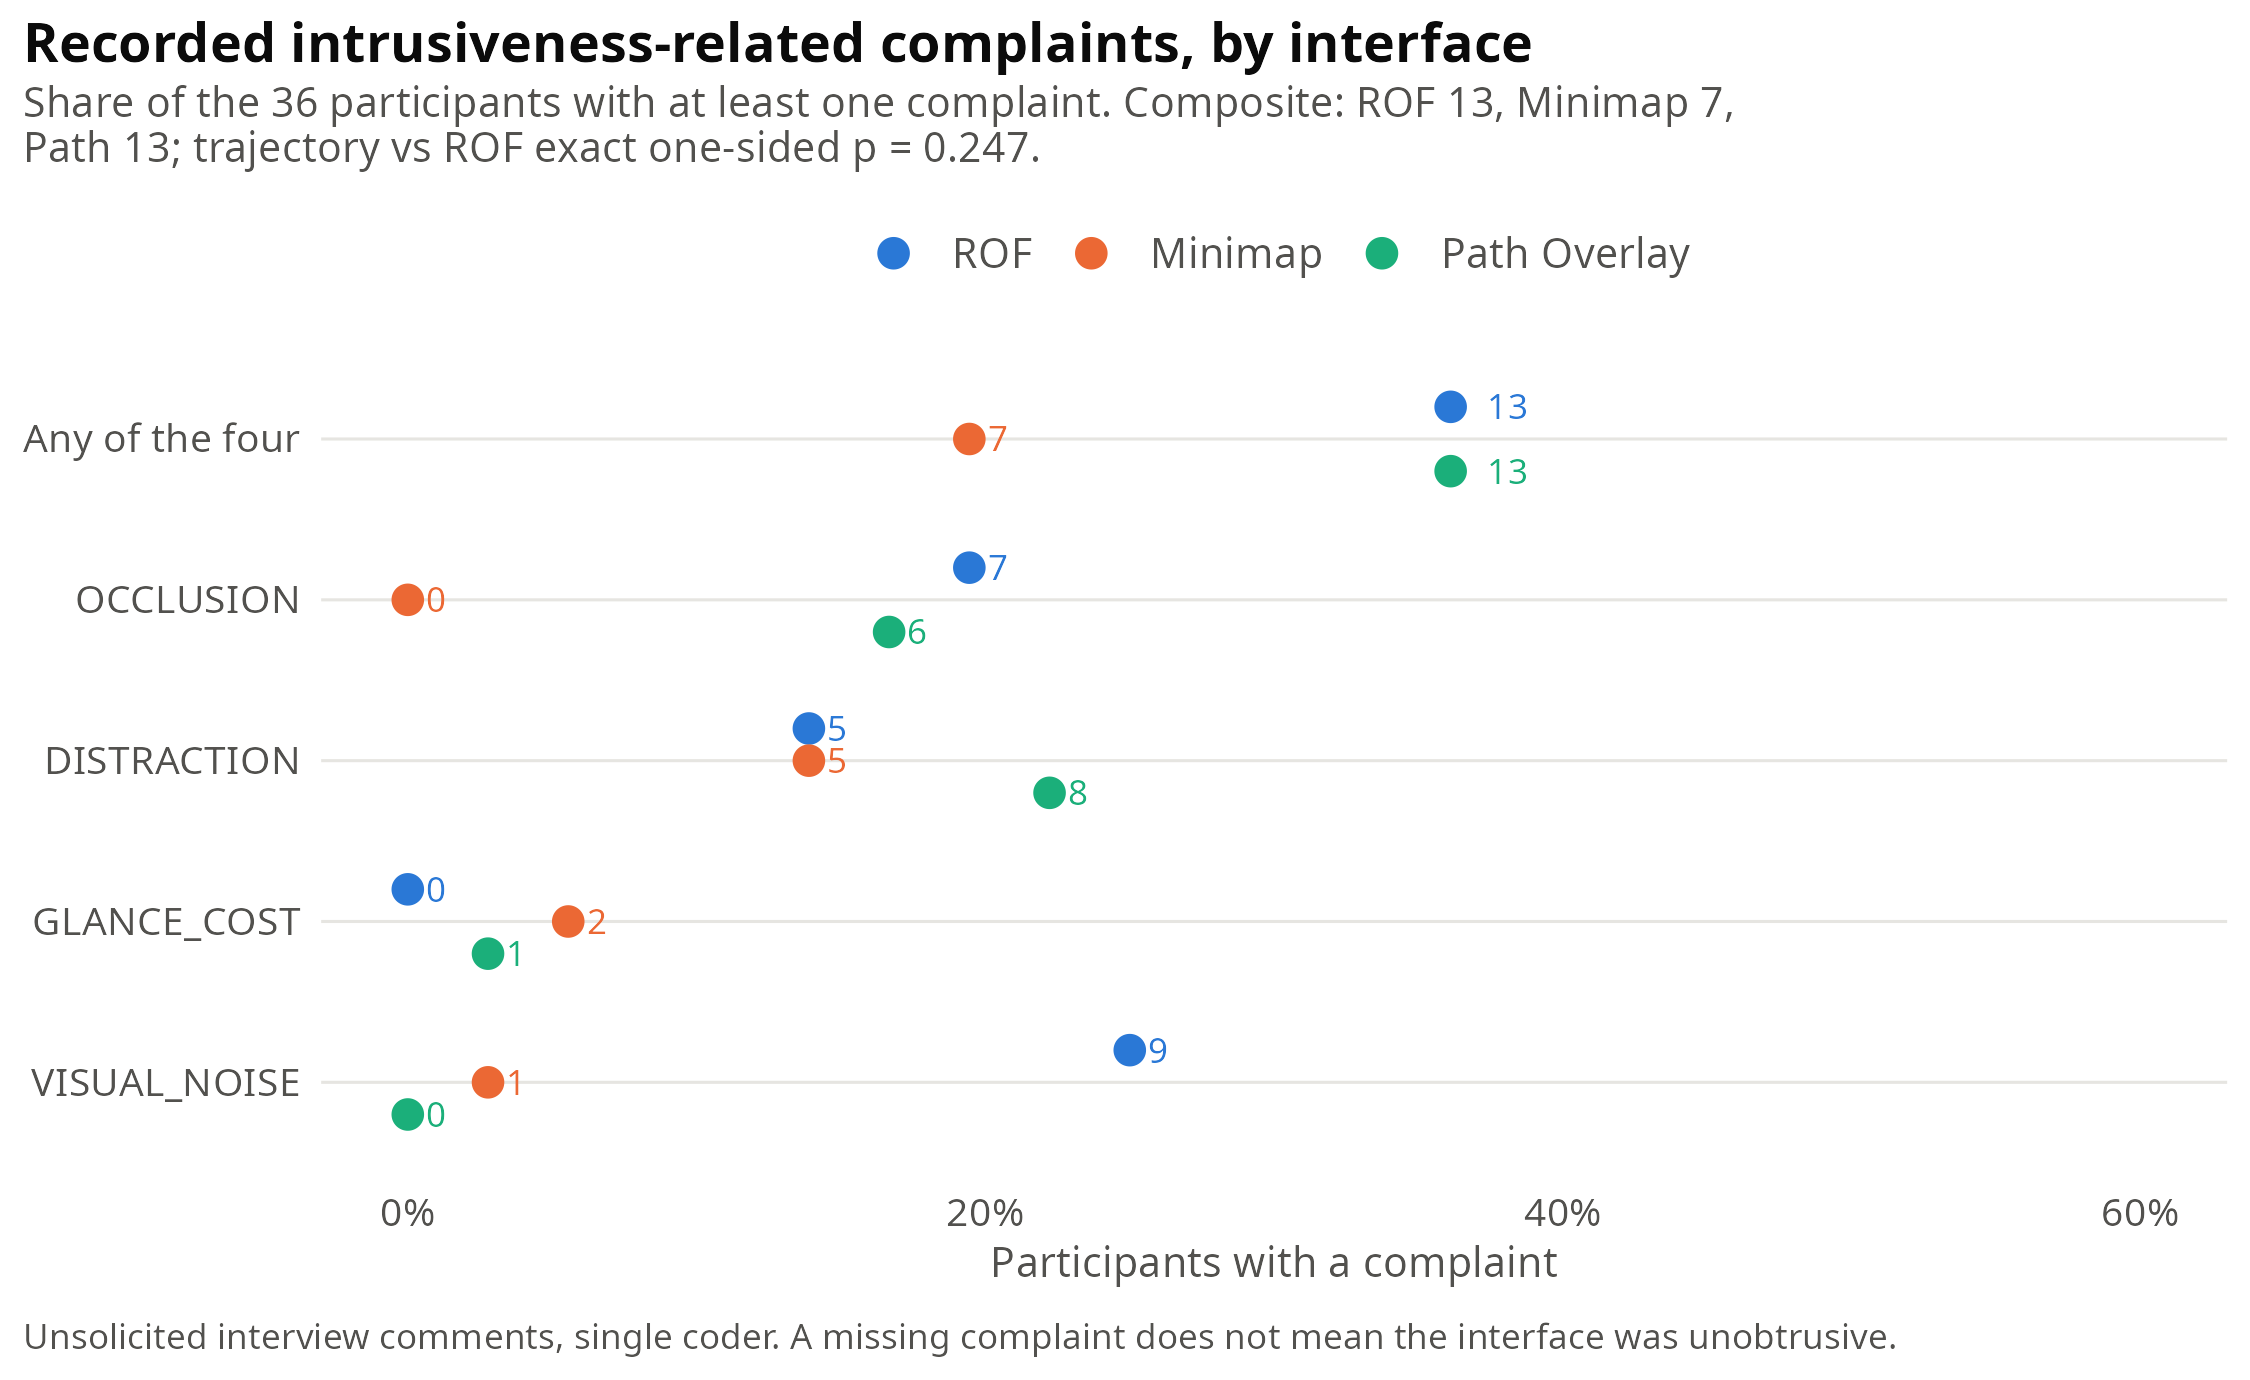
\includegraphics[width=0.8\textwidth]{figures/study2_complaints.png}
  \caption{Participants who made at least one recorded intrusiveness-related
  complaint about each method, overall (``any of the four'') and by complaint
  type. Counts are out of 36 participants.}
  \label{fig:s2-complaints}
\end{figure*}

\subsubsection{Preference Ranking}

Unlike in Study~1, all 36 participants provided a complete ranking
(Table~\ref{tab:s2-rank}). \textbf{No method was preferred overall}: the
rankings did not differ (Friedman $\chi^2(2) = 0.72$, $p = .697$), and
participants barely agreed with one another (Kendall's $W = .010$). ROF was
ranked last by 16 participants (44\%, 95\% CI [28, 62]), which was not more
often than expected by chance ($p = .11$). In the Plackett--Luce model, each
trajectory-based interface had an estimated probability of .36 of being ranked
first, compared with .27 for ROF, but this difference was not significant
(worth ratio 1.34, 95\% CI [0.78, 2.32], $p = .28$).

The secondary questions showed the same picture. Of the 21 participants who
named the method that best reduced their sickness, 8 chose ROF, 7 Minimap,
and 6 Overlay Path; of the 26 who named the most realistic method, 11 chose
ROF, 7 Minimap, and 8 Overlay Path.

When explaining their first choice, 86\% of participants referred to interface
experience, such as occlusion, distraction, or route anticipation, whereas only
19\% referred to sickness and 25\% to realism. \textbf{Participants' sense of
``balance'' therefore rested mainly on how each interface fit into the viewing
experience}, rather than on perceived sickness reduction.

\begin{table}[t]
  \caption{Preference ranking in Study~2 ($n = 36$). Lower mean rank indicates
  stronger preference. Borda score: 2 points for first place, 1 for second.}
  \label{tab:s2-rank}
  \centering
  \footnotesize
  \begin{tabular}{lcccc}
    \toprule
    \textbf{Method} & \textbf{Mean rank} & \textbf{Borda} & \textbf{First} & \textbf{Last} \\
    \midrule
    Overlay Path & \textbf{1.92} & \textbf{39} & \textbf{13} & \textbf{10} \\
    Minimap      & 1.97 & 37 & 11 & \textbf{10} \\
    ROF          & 2.11 & 32 & 12 & 16 \\
    \bottomrule
  \end{tabular}
\end{table}

\begin{table*}[t]
  \caption{Integration of quantitative and qualitative findings in Study~2.
  Interview counts are numbers of participants (out of 36).}
  \label{tab:s2-integration}
  \centering
  \footnotesize
  \begin{tabularx}{\textwidth}{lXX}
    \toprule
    \textbf{Method} & \textbf{Quantitative result} & \textbf{Interview feedback} \\
    \midrule
    Minimap      & TSC increased by 9.07; non-inferior to ROF (upper limit 2.71). Presence 5.12. &
                   Fewest intrusiveness-related complaints (7). Never described as blocking the scene; route preview valued (10). Some found it distracting (5) or forgot to look at it (5). \\
    Overlay Path & Numerically smallest TSC increase (7.24); non-inferior to ROF (upper limit 0.69). Presence 5.04. &
                   Most-cited advantage in the study: anticipating turns (17); seen as realistic (11). Most distraction complaints (8); too large or blocking the scene (6). \\
    ROF          & TSC increased by 9.00. Presence 5.10. &
                   Most often praised for realism (13), e.g., a ``wind effect''. Most complaints about flicker and visual clutter (9). Ranked last most often (16). \\
    \bottomrule
  \end{tabularx}
\end{table*}

\subsubsection{Study 2 Summary}

Table~\ref{tab:s2-integration} combines the quantitative and qualitative
results. Study~2 shows that \textbf{the trajectory-based interfaces were
non-inferior to ROF in measured VIMS}: sickness increased by a similar amount
under all three methods, and the data rule out the trajectory-based interfaces
being more than 0.84 TSC points worse than ROF on average. \textbf{Presence was
equally high for all three methods.} The data did \emph{not} show that the
trajectory-based interfaces were less intrusive: they drew about as many
recorded complaints as ROF, but of a different kind. ROF was criticized for
flicker, Overlay Path for distraction and occlusion, and Minimap drew the fewest
complaints. Participants did not agree on a single most balanced method; their
rankings followed these trade-offs rather than perceived sickness reduction.

These results have three limitations. First, Study~2 had no Baseline, so it
cannot show that any method reduced VIMS relative to unmodified video. Second,
sickness was mild (post-trial TSC 16.6--18.9, compared with 48.3--71.6 in
Study~1), which may have left little room for the methods to differ. Third,
the complaint analysis relies on unprompted comments coded by one researcher.
